\documentclass[aspectratio=169]{beamer}
\usetheme{Madrid}
\usecolortheme{default}

% Packages
\usepackage{graphicx}
\usepackage{amsmath}
\usepackage{amssymb}
\usepackage{tikz}
\usetikzlibrary{shapes,arrows,positioning}
\usepackage{hyperref}
\usepackage{algorithm}
\usepackage{algorithmic}
\usepackage{listings}

% Custom colors
\definecolor{themeblue}{RGB}{0,102,204}
\definecolor{themegreen}{RGB}{0,153,76}
\definecolor{themered}{RGB}{204,0,51}
\definecolor{themeorange}{RGB}{255,140,0}
\definecolor{themepurple}{RGB}{148,0,211}

\setbeamercolor{structure}{fg=themeblue}
\setbeamercolor{alerted text}{fg=themered}
\setbeamercolor{example text}{fg=themegreen}

% Title information
\title{Your Presentation Title}
\subtitle{Your Subtitle Here}
\author{Your Name}
\institute{Your Institution}
\date{\today}

% Footer customization
\setbeamertemplate{footline}[frame number]

\begin{document}

% Title slide
\begin{frame}
    \titlepage
\end{frame}

% Table of contents with animation
\begin{frame}{Outline}
    \tableofcontents[pausesections]
\end{frame}

\section{Animation Techniques}

\subsection{Basic Animations}

\begin{frame}{Technique 1: Progressive Reveal with \textbackslash pause}
    This is the simplest animation technique.
    \pause
    
    Content appears when you advance the slide.
    \pause
    
    Perfect for:
    \pause
    \begin{itemize}
        \item Simple step-by-step reveals
        \pause
        \item Quick presentations
        \pause
        \item Linear storytelling
    \end{itemize}
    \pause
    
    \alert{Use sparingly for best effect!}
\end{frame}

\begin{frame}{Technique 2: Overlay Specifications}
    % Demonstrates <n->, <n>, <n-m> syntax
    
    \textbf<1>{This text is bold only on slide 1}
    
    \textcolor<2>{themered}{This text is red only on slide 2}
    
    \begin{itemize}
        \item<1-> Visible from slide 1 onwards
        \item<2-> Visible from slide 2 onwards
        \item<3-> Visible from slide 3 onwards
        \item<4-5> Only visible on slides 4 and 5
        \item<6-> Final item from slide 6
    \end{itemize}
    
    \onslide<7->{
        \begin{block}{Summary}
            Overlay specifications give you precise control over when elements appear!
        \end{block}
    }
\end{frame}

\begin{frame}{Technique 3: Incremental Lists [<+->]}
    Without manual numbering, you can create progressive lists:
    
    \begin{itemize}[<+->]
        \item First item appears
        \item Then second item
        \item Then third item
        \item Fourth item follows
        \item And finally the fifth
    \end{itemize}
    
    \vspace{1em}
    
    Works with enumerate too:
    \begin{enumerate}[<+->]
        \item Step one
        \item Step two
        \item Step three
    \end{enumerate}
\end{frame}

\begin{frame}{Technique 4: TikZ Animations}
    % Demonstrate animated TikZ graphics
    TikZ graphics can be animated using overlay specifications:
    
    \vspace{1em}
    
    \begin{center}
        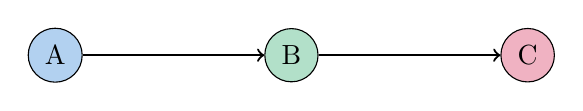
\begin{tikzpicture}[scale=1.5]
            \node<1->[draw, circle, fill=themeblue!30] (a) at (0,0) {A};
            \node<2->[draw, circle, fill=themegreen!30] (b) at (2,0) {B};
            \node<3->[draw, circle, fill=themered!30] (c) at (4,0) {C};
            \draw<4->[->, thick] (a) -- (b);
            \draw<5->[->, thick] (b) -- (c);
        \end{tikzpicture}
    \end{center}
    
    \vspace{1em}
    
    \begin{itemize}
        \item<1-> Node A appears first
        \item<2-> Then node B
        \item<3-> Then node C
        \item<4-> Edge A→B appears
        \item<5-> Finally edge B→C appears
    \end{itemize}
\end{frame}

\begin{frame}[fragile]{Technique 5: Content Replacement with \textbackslash only}
    % Demonstrate different approaches
    \begin{itemize}
        \item<1-> First key point about your topic
        \item<2-> Second important aspect to highlight
        \item<3-> Third critical element to discuss
        \item<4-> \alert{Key takeaway or innovation}
    \end{itemize}
    
    \vspace{1em}
    
    \onslide<5->{
        \begin{block}{Main Goal}
            Your main objective or key message
        \end{block}
    }
\end{frame}

\begin{frame}{Comparison Example}
    % Using \only for replacement animation
    \only<1>{
        \begin{center}
            \Large Comparing Two Approaches
        \end{center}
    }
    \only<2->{
        \begin{columns}
            \column{0.5\textwidth}
            \begin{block}{Traditional Approach}
                \begin{itemize}
                    \item First characteristic
                    \item Second characteristic
                    \item Third characteristic
                \end{itemize}
            \end{block}
            
            \column{0.5\textwidth}
            \begin{block}{Your Approach}
                \begin{itemize}
                    \item<3-> Improved feature one
                    \item<4-> Improved feature two
                    \item<5-> Improved feature three
                \end{itemize}
            \end{block}
        \end{columns}
    }
\end{frame}

\section{Background}

\begin{frame}{Key Concepts}
    % Alert animation
    \begin{definition}<1->
        A \alert<1>{key term} is defined here with proper context.
    \end{definition}
    
    \vspace{1em}
    
    % Incremental list with custom animations
    \begin{itemize}[<+->]
        \item First concept: brief explanation
        \item Second concept: brief explanation
        \item Third concept: brief explanation
        \item Challenge: main problem to solve
    \end{itemize}
\end{frame}

\begin{frame}{Mathematical Example}
    % Math with animations
    \begin{align}
        \onslide<1->{f(x) &= \int_0^x g(t) dt \\}
        \onslide<2->{f'(x) &= g(x) \\}
        \onslide<3->{f''(x) &= g'(x)}
    \end{align}
    
    \vspace{1em}
    
    \onslide<4->{
        \begin{alertblock}{Key Insight}
            Your key mathematical or conceptual insight goes here!
        \end{alertblock}
    }
\end{frame}

\section{Methodology}

\begin{frame}{Your Algorithm/Process}
    % Uncovering animation for algorithm steps
    \begin{enumerate}
        \item<1-> Step one: initial setup or preparation
        \item<2-> Step two: main processing or computation
        \item<3-> Step three: refinement or optimization
        \item<4-> Step four: validation or verification
        \item<5-> Step five: final output or results
    \end{enumerate}
    
    \vspace{1em}
    
    \visible<6->{
        \begin{center}
            \tikz{
                \node[draw, rectangle, fill=themeblue!20] (eg) at (0,0) {Input};
                \node[draw, rectangle, fill=themegreen!20] (se) at (3,0) {Process};
                \node[draw, rectangle, fill=themered!20] (opt) at (6,0) {Output};
                \draw[->, thick] (eg) -- (se);
                \draw[->, thick] (se) -- (opt);
            }
        \end{center}
    }
\end{frame}

\begin{frame}{Visual Demonstration}
    % Multiple overlays with different content
    \begin{center}
        \only<1>{
            \tikz{
                \node[draw, circle] (a) at (0,0) {A};
                \node[draw, circle] (b) at (2,0) {B};
                \node[draw, circle] (c) at (1,1) {C};
                \draw[->] (c) -- (a);
                \draw[->] (c) -- (b);
            }
            
            \vspace{0.5em}
            Stage 1: Basic Structure
        }
        \only<2>{
            \tikz{
                \node[draw, circle, fill=themeblue!20] (e1) at (0,0) {A};
                \node[draw, circle, fill=themegreen!20] (e2) at (3,0) {B};
                \node at (0,-1) {Component 1};
                \node at (3,-1) {Component 2};
            }
            
            \vspace{0.5em}
            Stage 2: With Components
        }
        \only<3>{
            \tikz{
                \node[draw, circle, fill=themered!30, minimum size=1.5cm] (soft) at (1.5,0) {Final};
                \node at (1.5,-1) {Integrated Result};
                \node at (1.5,-1.7) {\small complete system};
            }
            
            \vspace{0.5em}
            Stage 3: Final Result
        }
    \end{center}
\end{frame}

\section{Results}

\begin{frame}{Your Results}
    % Animated appearance
    \begin{columns}
        \column{0.5\textwidth}
        \onslide<1->{
            \textbf{Test Cases:}
            \begin{itemize}
                \item<2-> Test case one
                \item<3-> Test case two
                \item<4-> Test case three
            \end{itemize}
        }
        
        \column{0.5\textwidth}
        \onslide<5->{
            \textbf{Outcomes:}
            \begin{itemize}
                \item<6-> Positive result one
                \item<7-> Positive result two
                \item<8-> Positive result three
            \end{itemize}
        }
    \end{columns}
    
    \vspace{2em}
    
    \onslide<9->{
        \begin{exampleblock}{Performance}
            Your key performance metric or achievement!
        \end{exampleblock}
    }
\end{frame}

\begin{frame}{Comparison Table}
    % Animated table
    \begin{table}
        \centering
        \begin{tabular}{l|c|c|c}
            \textbf{Method} & \textbf{Metric 1} & \textbf{Metric 2} & \textbf{Metric 3} \\
            \hline
            \onslide<2->{Method A & Value 1 & Value 2 & Value 3 \\}
            \onslide<3->{Method B & Value 1 & Value 2 & Value 3 \\}
            \onslide<4->{\alert{Your Method} & \alert{Value 1} & \alert{Value 2} & \alert{Value 3} \\}
        \end{tabular}
        \caption{Comparison of different approaches}
    \end{table}
\end{frame}

\section{Conclusion}

\begin{frame}{Key Takeaways}
    % Emphasis animation
    \begin{enumerate}
        \item<1-> \textbf<1>{First key takeaway or finding}
        \item<2-> \textbf<2>{Second important conclusion}
        \item<3-> \textbf<3>{Third significant result}
        \item<4-> \textbf<4>{Fourth main implication or impact}
    \end{enumerate}
    
    \vspace{2em}
    
    \onslide<5->{
        \begin{center}
            \Large \alert{Thank you for your attention!}
        \end{center}
    }
\end{frame}

\begin{frame}{Future Work}
    % Transitional animation
    \transdissolve<1>
    
    \begin{block}{Planned Extensions}<2->
        \begin{itemize}
            \item Extension or improvement one
            \item Extension or improvement two
            \item Extension or improvement three
        \end{itemize}
    \end{block}
    
    \begin{block}{Open Questions}<3->
        \begin{itemize}
            \item Research question one?
            \item Research question two?
            \item Research question three?
        \end{itemize}
    \end{block}
\end{frame}

\begin{frame}[plain]
    % Final slide with custom appearance
    \begin{center}
        {\Huge Questions?}
        
        \vspace{2em}
        
        \onslide<2->{
            \normalsize
            Contact: your.email@institution.edu\\
            Website: your-website.com
        }
    \end{center}
\end{frame}

\end{document}
